\documentclass{article}
\usepackage[utf8]{inputenc}
\usepackage[english]{babel}

% pacchetto Multicolonna
\usepackage{multicol}
% pacchetto Immagine
\usepackage{graphicx} 

% inizio del documento
\begin{document}
% Titolo, Autore, Data.
\title{Prova Disegno}
\author{Luca Spanedda}
\date{\today}
%...
\maketitle
% --------------------------------------------------------------------------------
% --------------------------------------------------------------------------------
% --------------------------------------------------------------------------------
% --------------------------------------------------------------------------------

% per inserire un immagine in Latex la modalità è la seguente:

% immagine da inserire
\begin{figure}[h!] % inizio inserimento della figura
\begin{center} % posizionamento della figura centrale nel testo

  % Metto la figura: grandezza e nomefile.formato puntato nella stessa cartella
  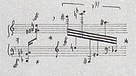
\includegraphics[width=12cm]{serenata.jpg}\\ 
   % scrittura sotto l'immagine
  \caption{Estratto da una partitura di Bruno Maderna} 
\end{center} % finisco posizionamento della figura centrale
\end{figure} % finisco inserimento della figura
% ----------------------------------------


\end{document}